\documentclass[12pt, oneside]{article}   	% use "amsart" instead of "article" for
\usepackage[left=2.7cm,right=2.7cm,top=2.7cm,bottom=2.7cm]{geometry}	
\usepackage{amsmath}
\usepackage{graphicx}
\usepackage{float}
\usepackage{fancyvrb}
\usepackage{lipsum}
\usepackage{xcolor}
\usepackage{subcaption}

\setlength{\parindent}{0pt}
\newcommand{\reffig}[1]{Figure \ref{#1}\hspace{2pt}}
\newcommand{\reftab}[1]{Table \ref{#1}\hspace{2pt}}

\begin{document}
\title{Project 3}
\author{Kun Zhou}
\date{\today}
\maketitle
P1\\
The graphs are on page 2,3.
\begin{itemize}
  \item When $\beta$ becomes larger, more sweeps are needed to make $H(X)$ converge to $h^*$.
  \item When $\beta$ becomes larger, $h^*$ become smaller.
  \item It's hard to say which version of method is better. But based on the graphs, version 2 is better.
  \item Obviously, checkerboard image starts $h$ from 1 while constant image starts from $0$.
\end{itemize}
P2\\
It's hard to display the sweeps for Gibbs Sampler since the sweeps are too large. So I show it in the following table.
\begin{table}
\center
\begin{tabular}{|ccccccc|}
  \hline
  % after \\: \hline or \cline{col1-col2} \cline{col3-col4} ...\multicolum
   & \multicolumn{6}{c|}{$\beta$} \\ \hline
   & \multicolumn{2}{c}{0.65} & \multicolumn{2}{c}{0.75} & \multicolumn{2}{c|}{0.85} \\
   & MC1 & MC2 &MC1 & MC2 &MC1 & MC2 \\\hline
   Version 1 & 6 & 7 & 12 & 23 & 32 & 25\\
   Version 2 & 5.01 & 8.85 & 9.52 & 16.17 & 17.12 & 25.54 \\
   Gibbs & 54 & 54 & 158 & 158 & 1740 & 1740\\
  \hline
\end{tabular}
\end{table}


\begin{figure}[H]
        \centering
        \begin{subfigure}[b]{0.475\textwidth}
            \centering
            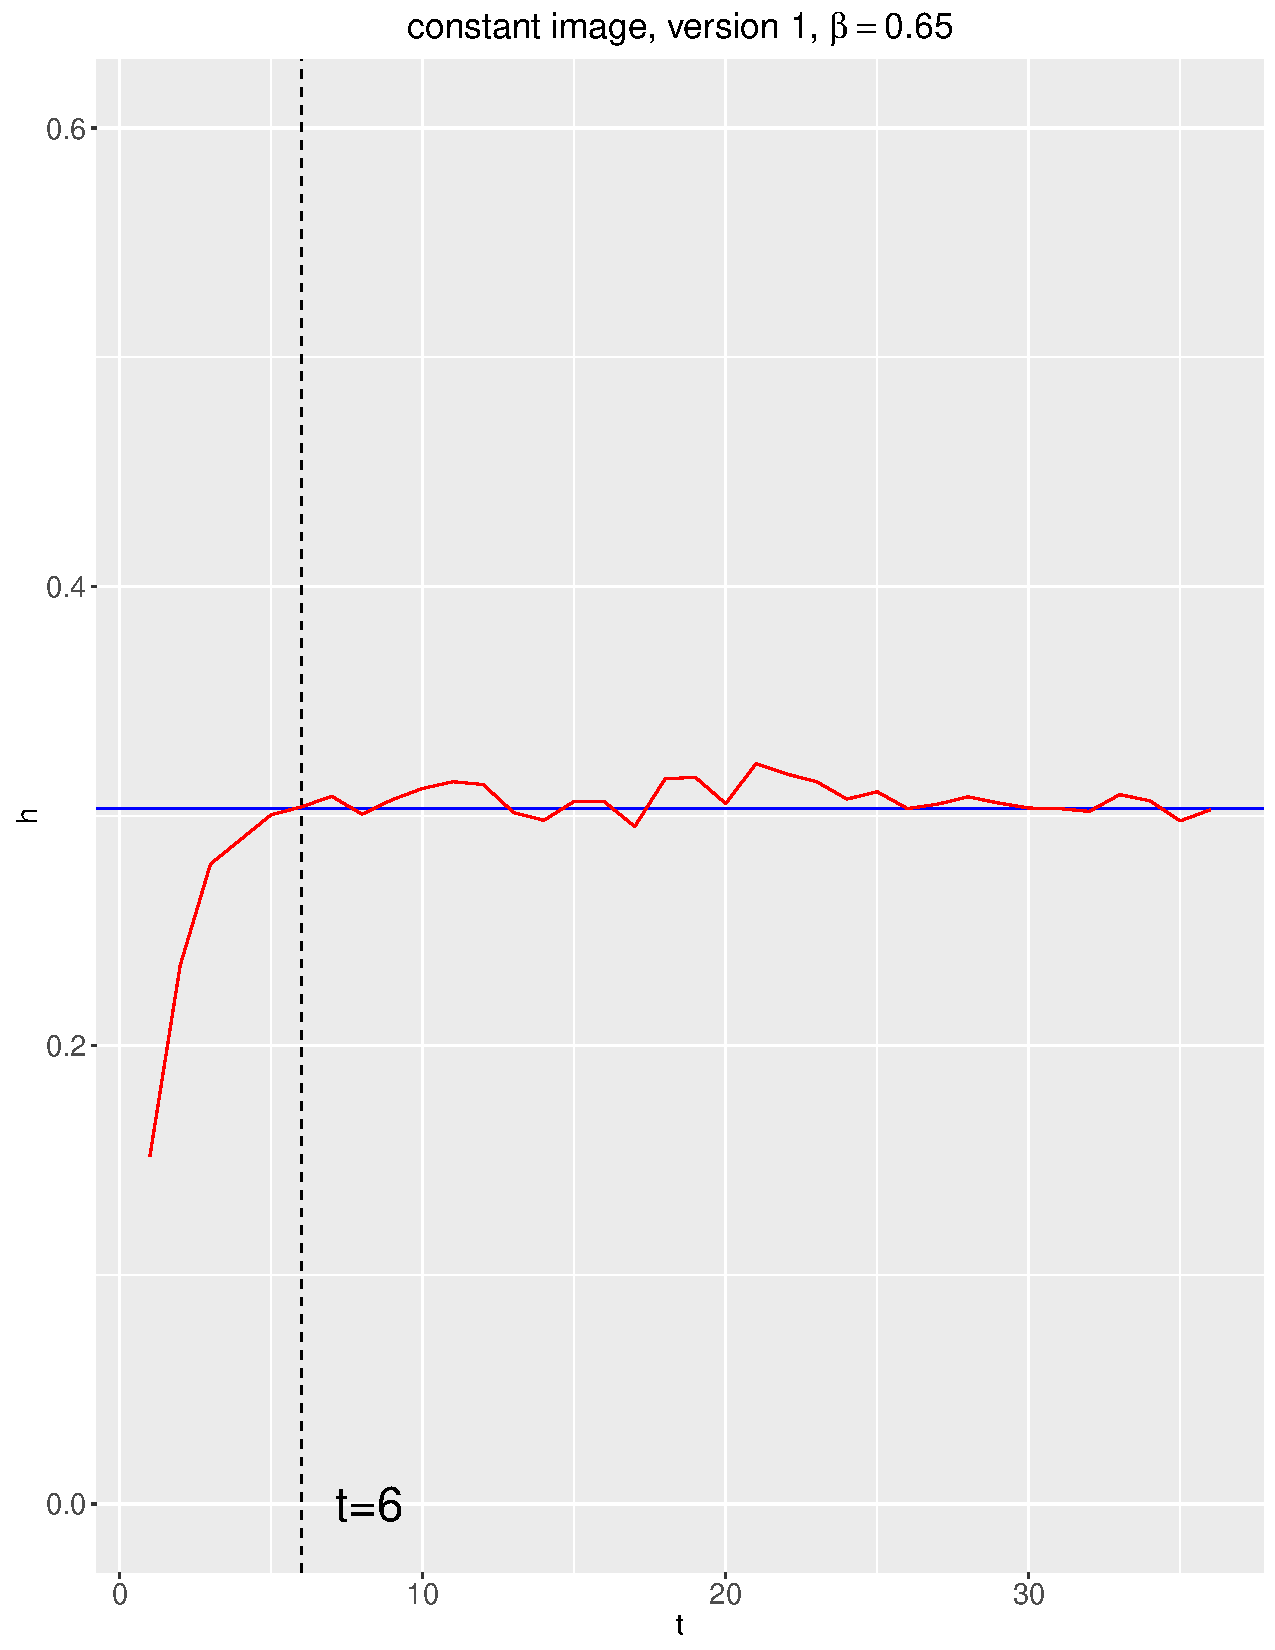
\includegraphics[width=\textwidth, height=0.32\textheight]{const_v1_65.pdf}
        \end{subfigure}
        \quad
        \begin{subfigure}[b]{0.475\textwidth}
            \centering
            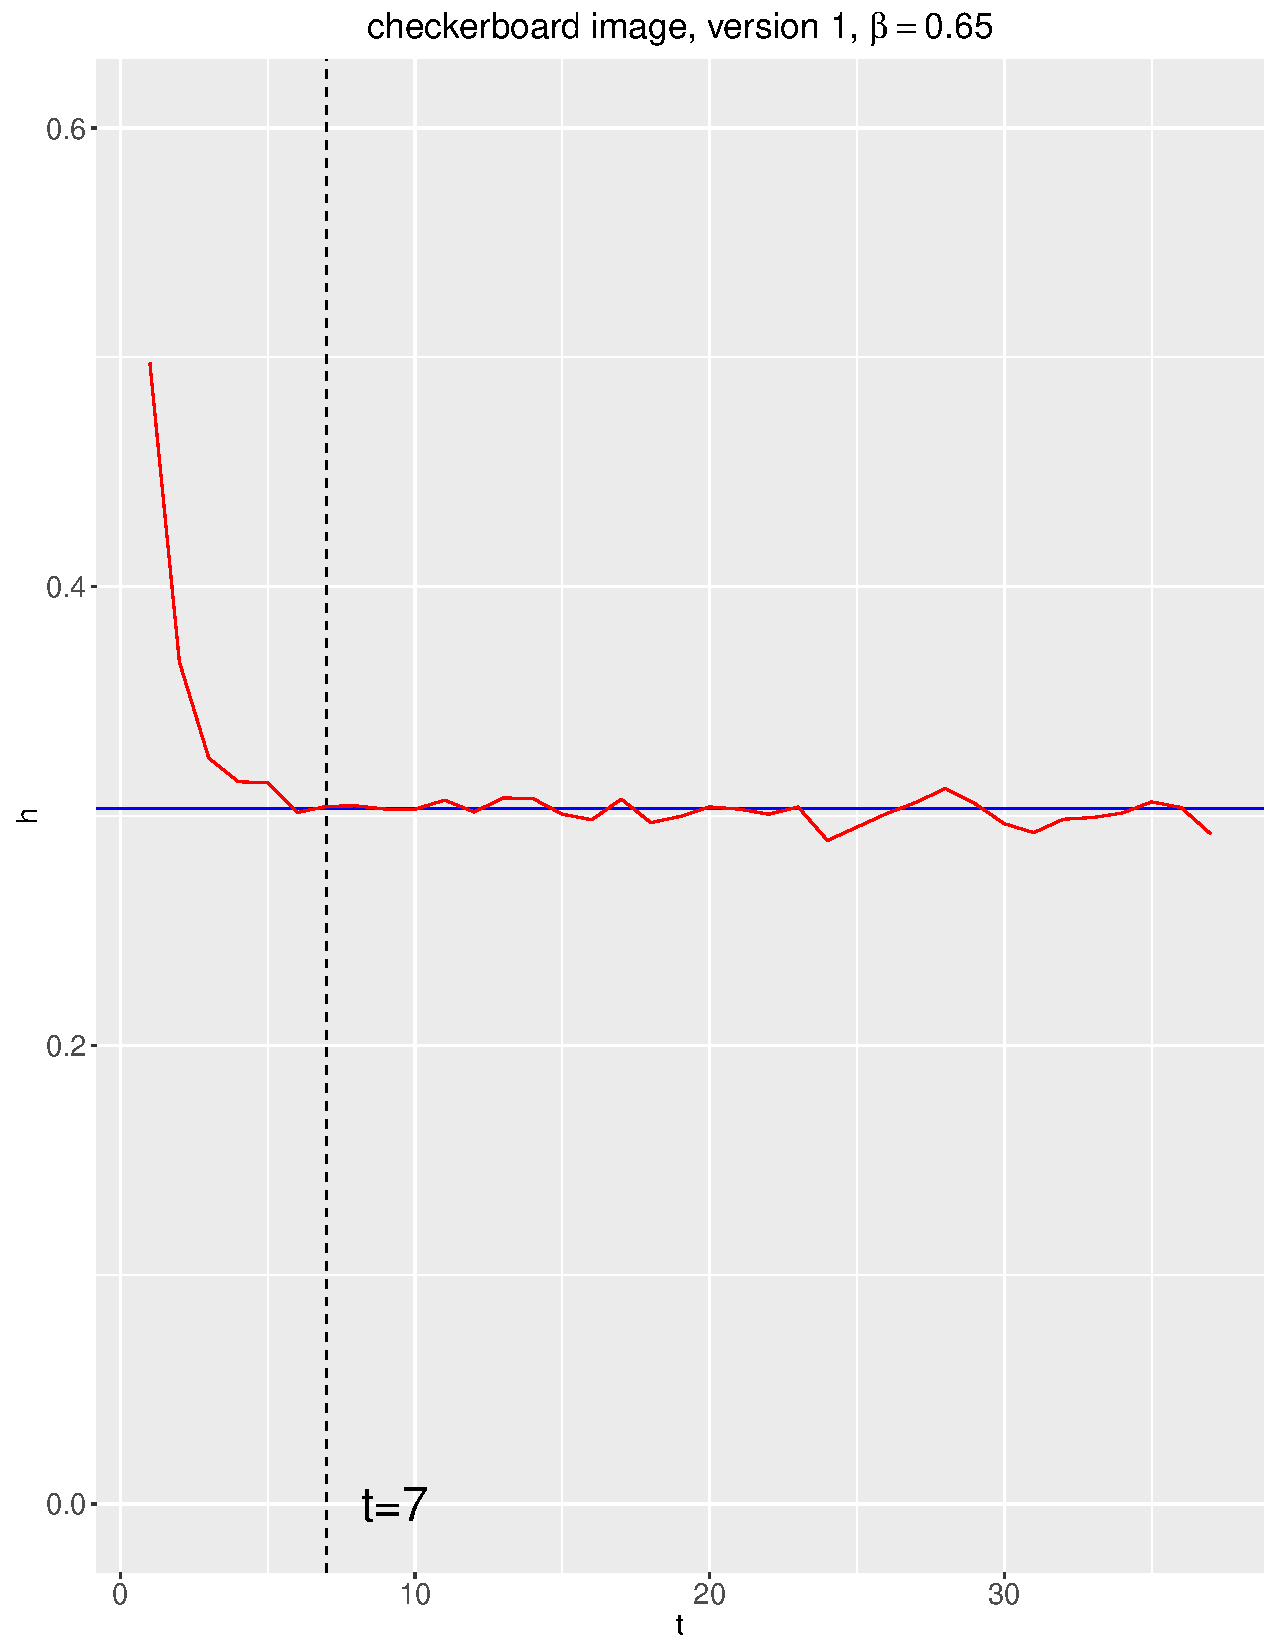
\includegraphics[width=\textwidth, height=0.32\textheight]{check_v1_65.pdf}
        \end{subfigure} \\
        \centering
        \begin{subfigure}[b]{0.475\textwidth}
            \centering
            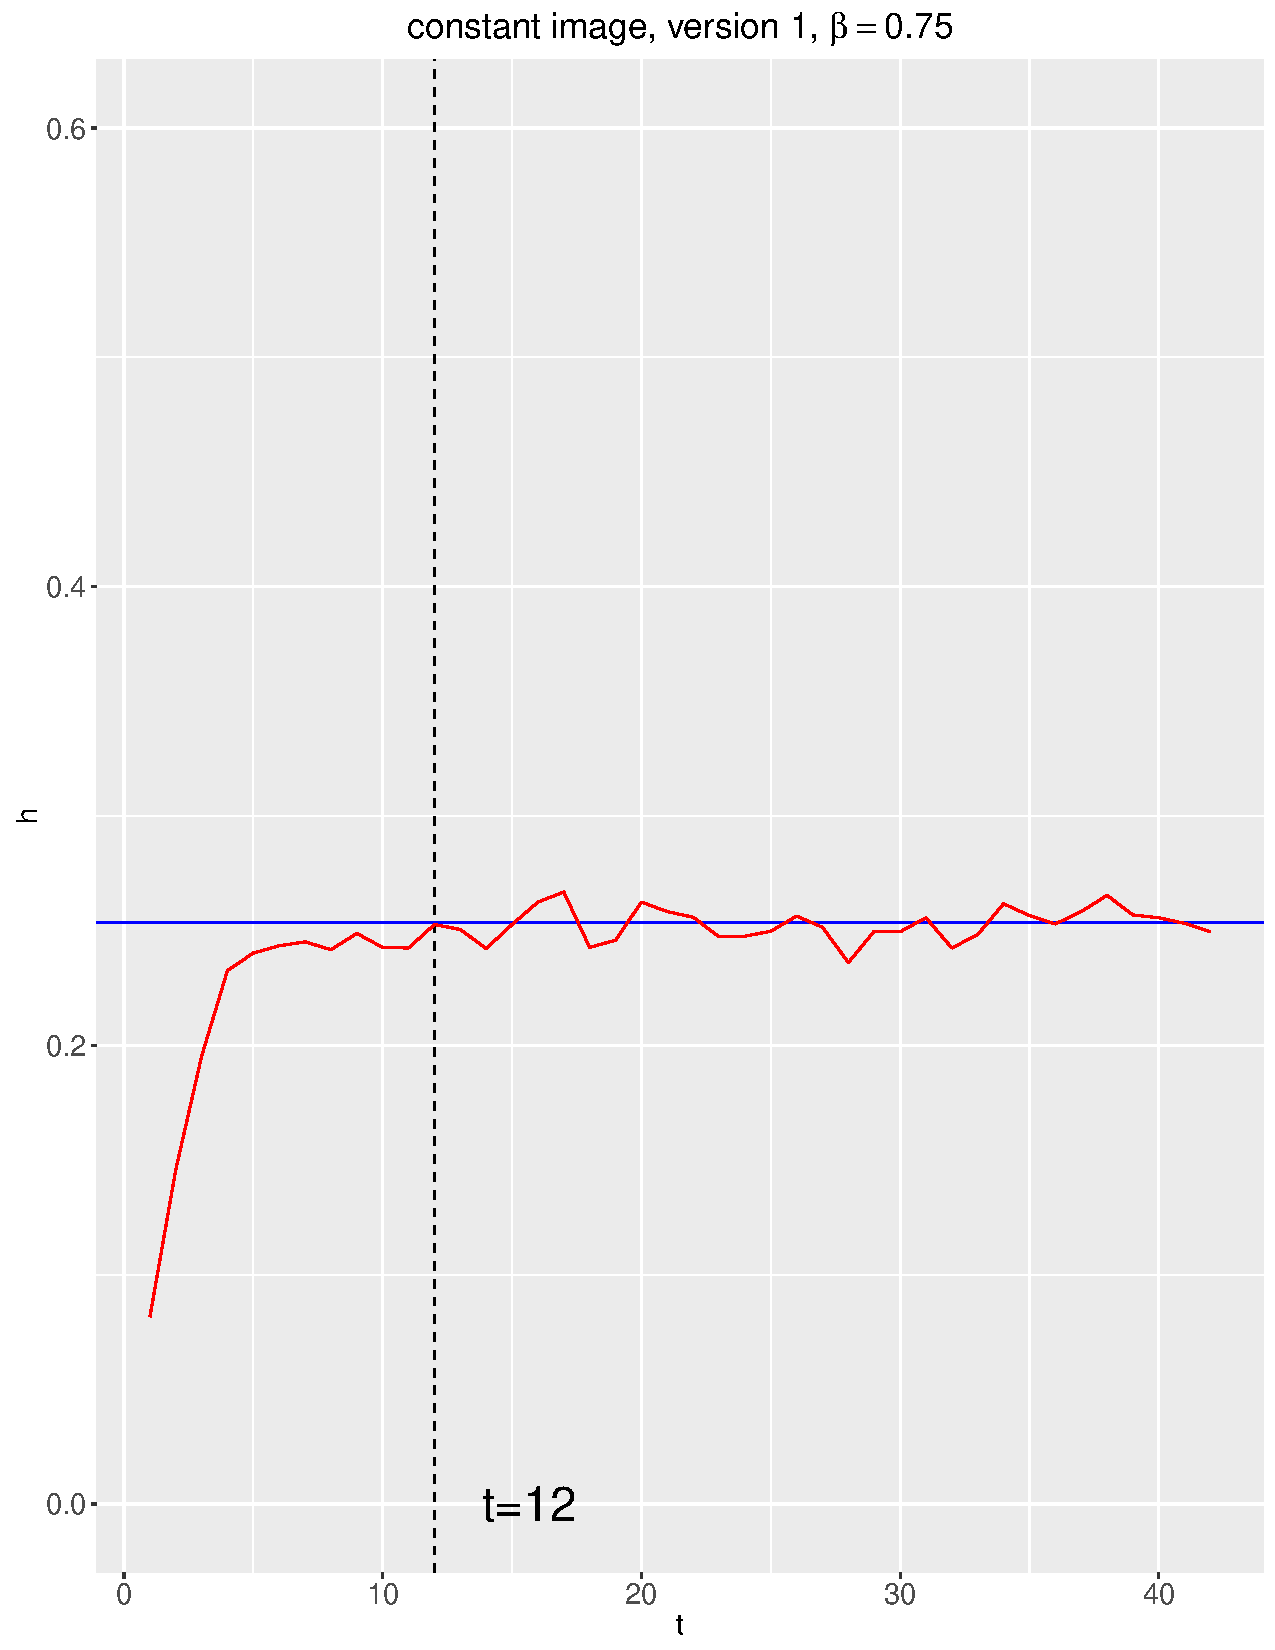
\includegraphics[width=\textwidth, height=0.32\textheight]{const_v1_75.pdf}
        \end{subfigure}
        \quad
        \begin{subfigure}[b]{0.475\textwidth}
            \centering
            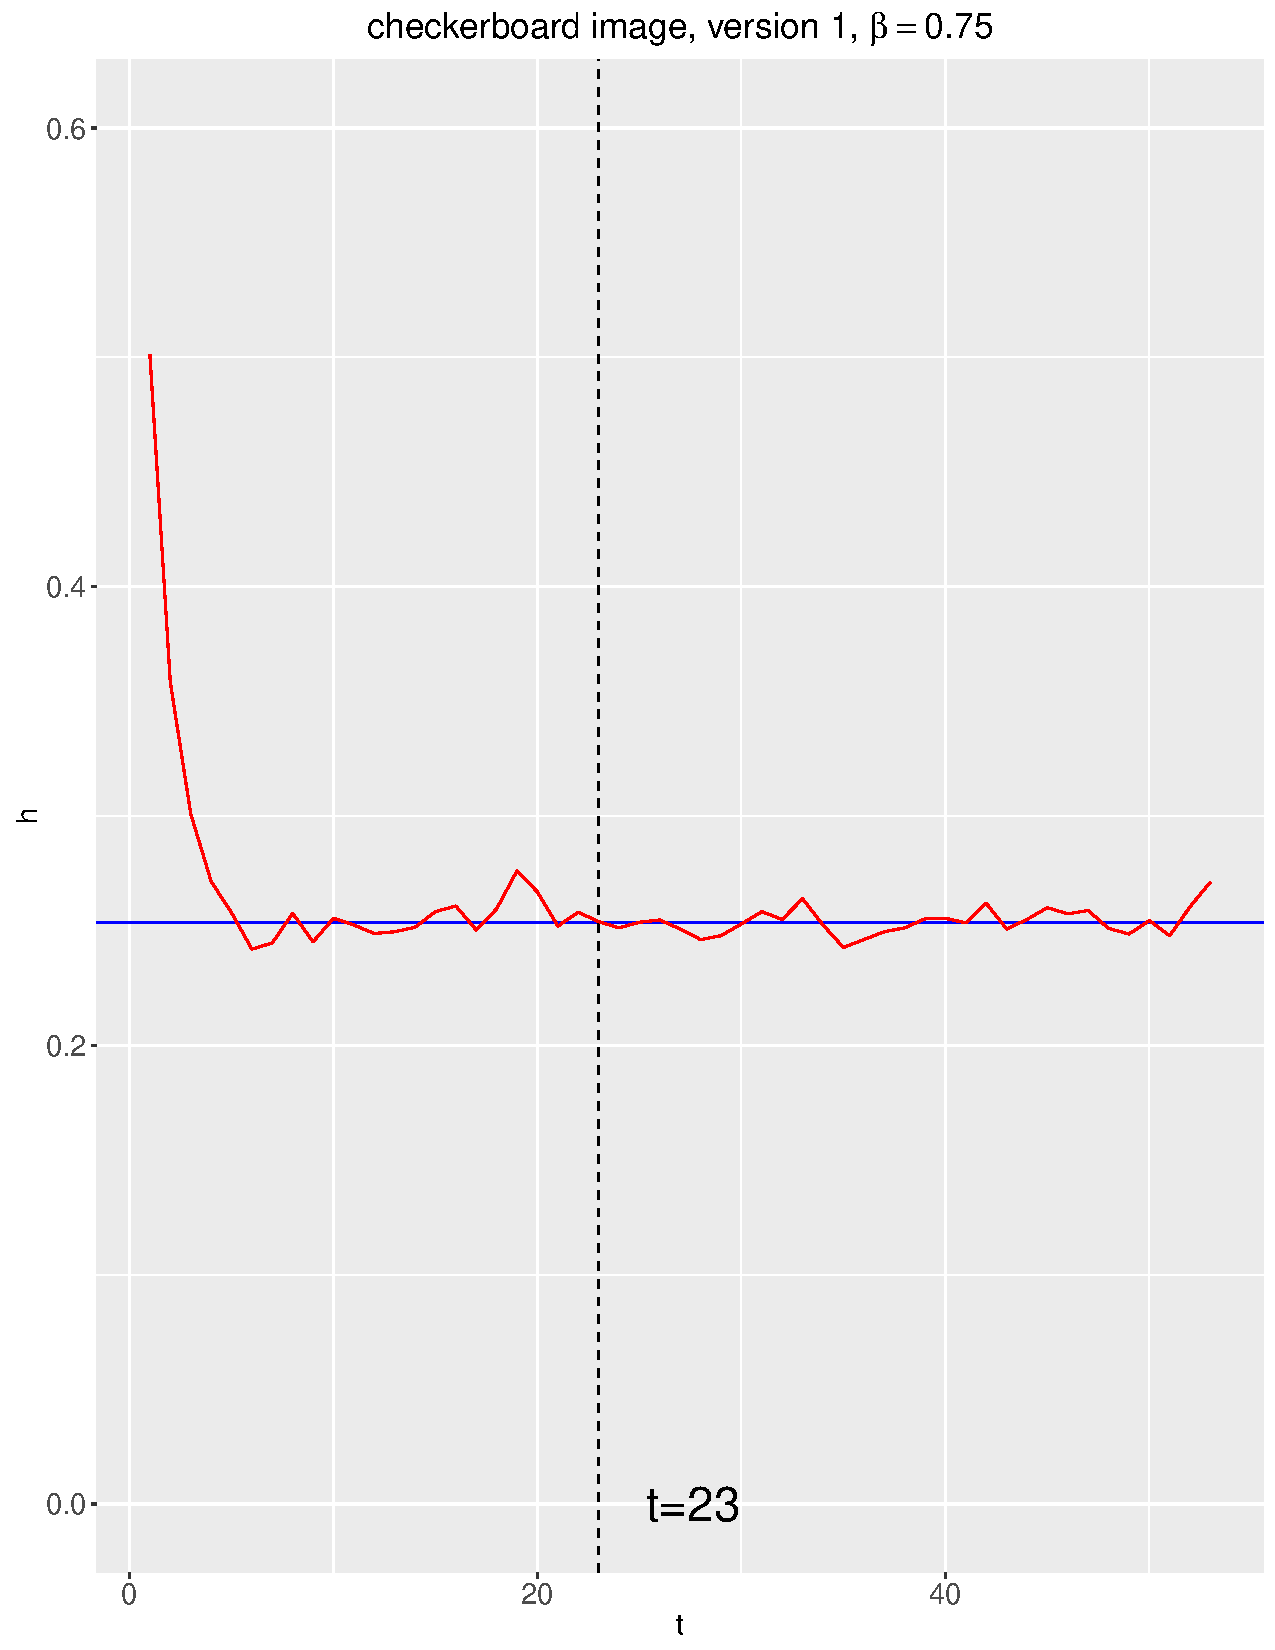
\includegraphics[width=\textwidth, height=0.32\textheight]{check_v1_75.pdf}
        \end{subfigure} \\
        \begin{subfigure}[b]{0.475\textwidth}
            \centering
            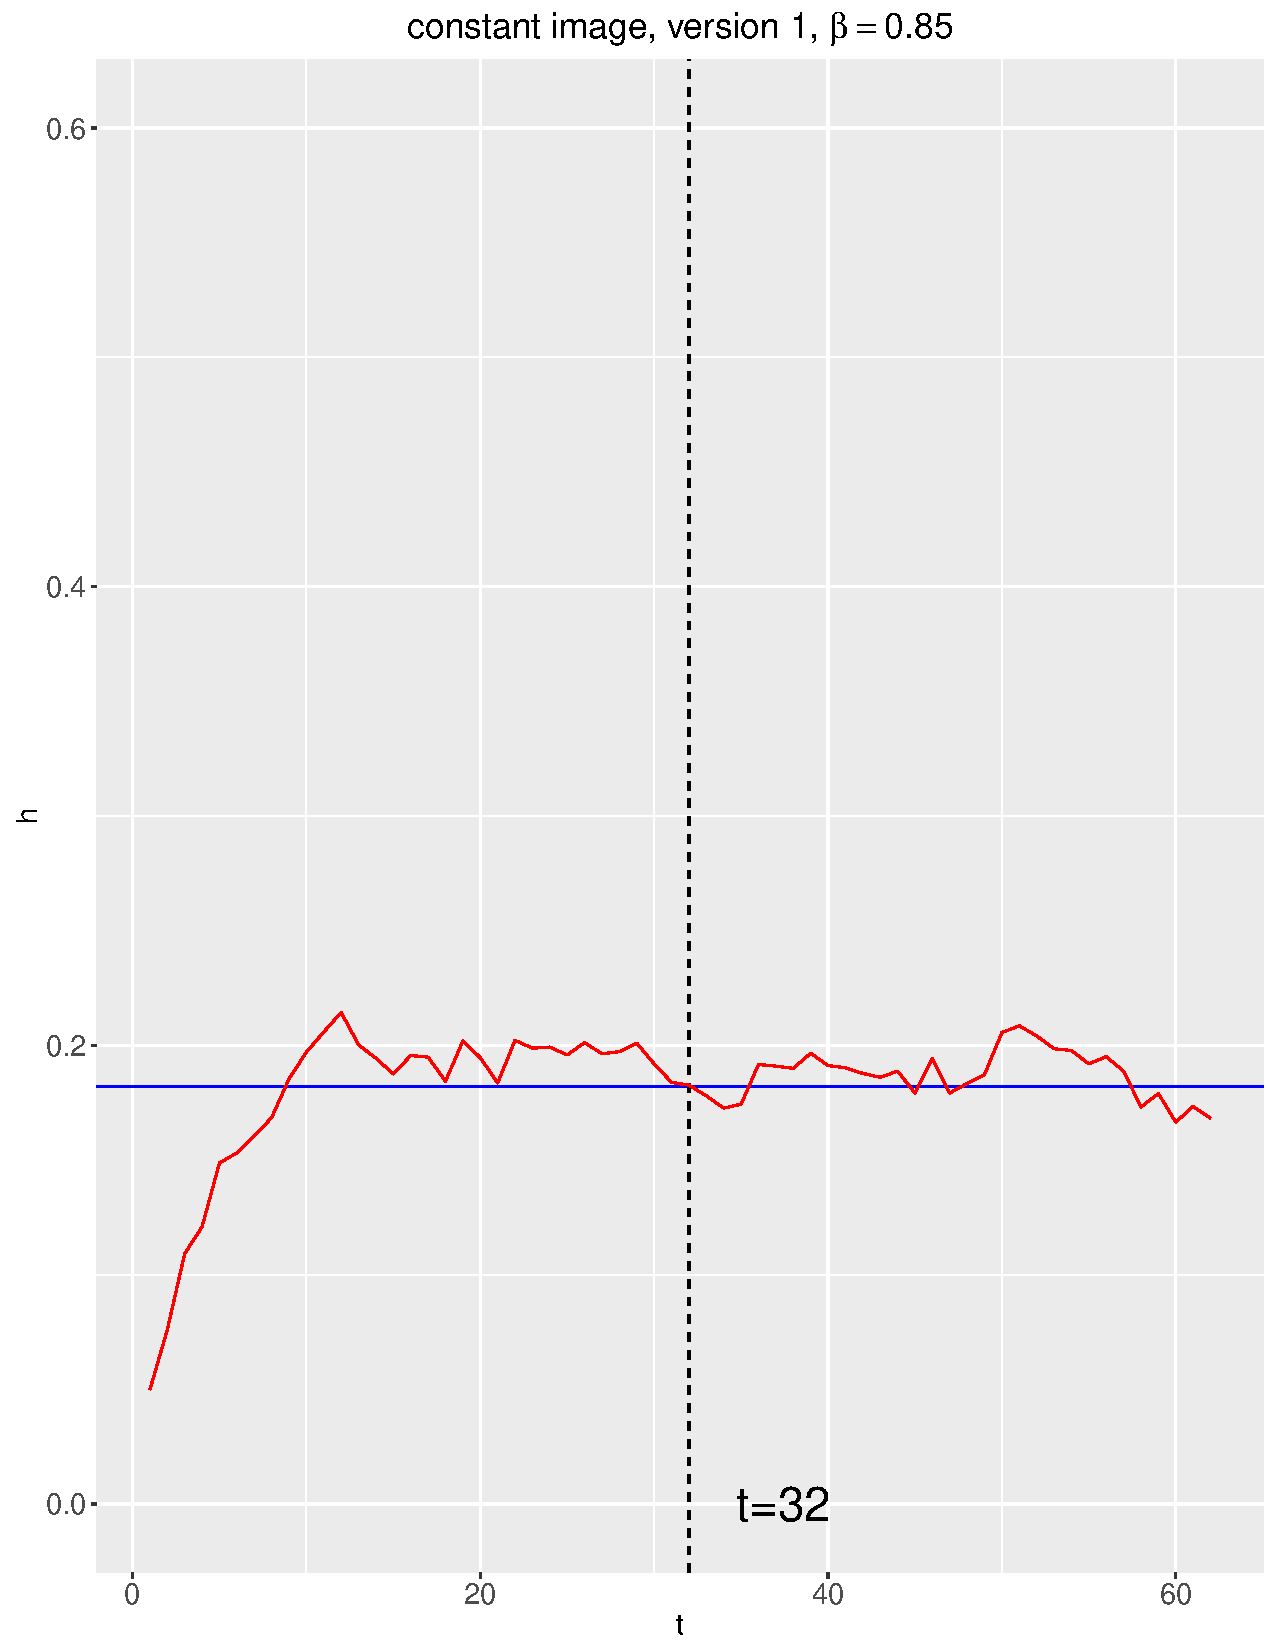
\includegraphics[width=\textwidth, height=0.32\textheight]{const_v1_85.pdf}
        \end{subfigure}
        \quad
        \begin{subfigure}[b]{0.475\textwidth}
            \centering
            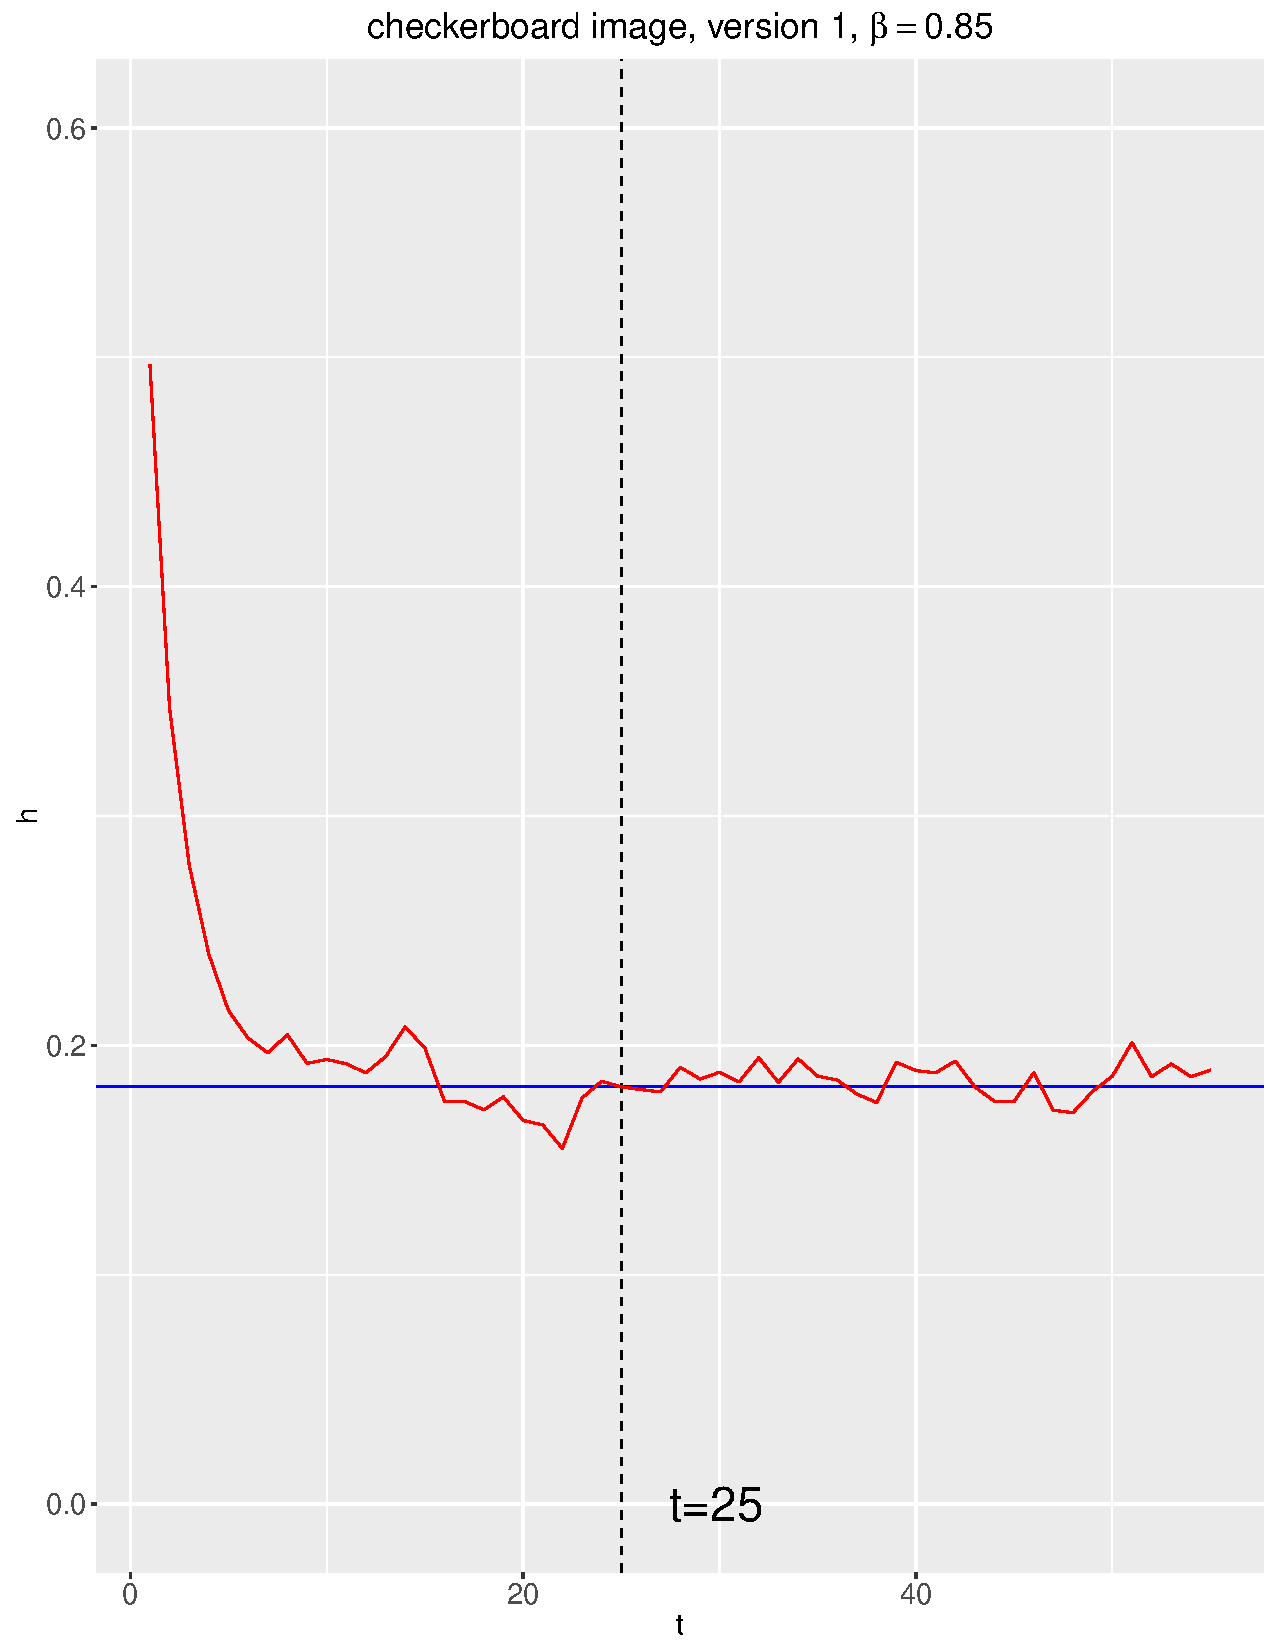
\includegraphics[width=\textwidth, height=0.32\textheight]{check_v1_85.pdf}
        \end{subfigure} \
\end{figure}
\begin{figure}[H]
        \centering
        \begin{subfigure}[b]{0.475\textwidth}
            \centering
            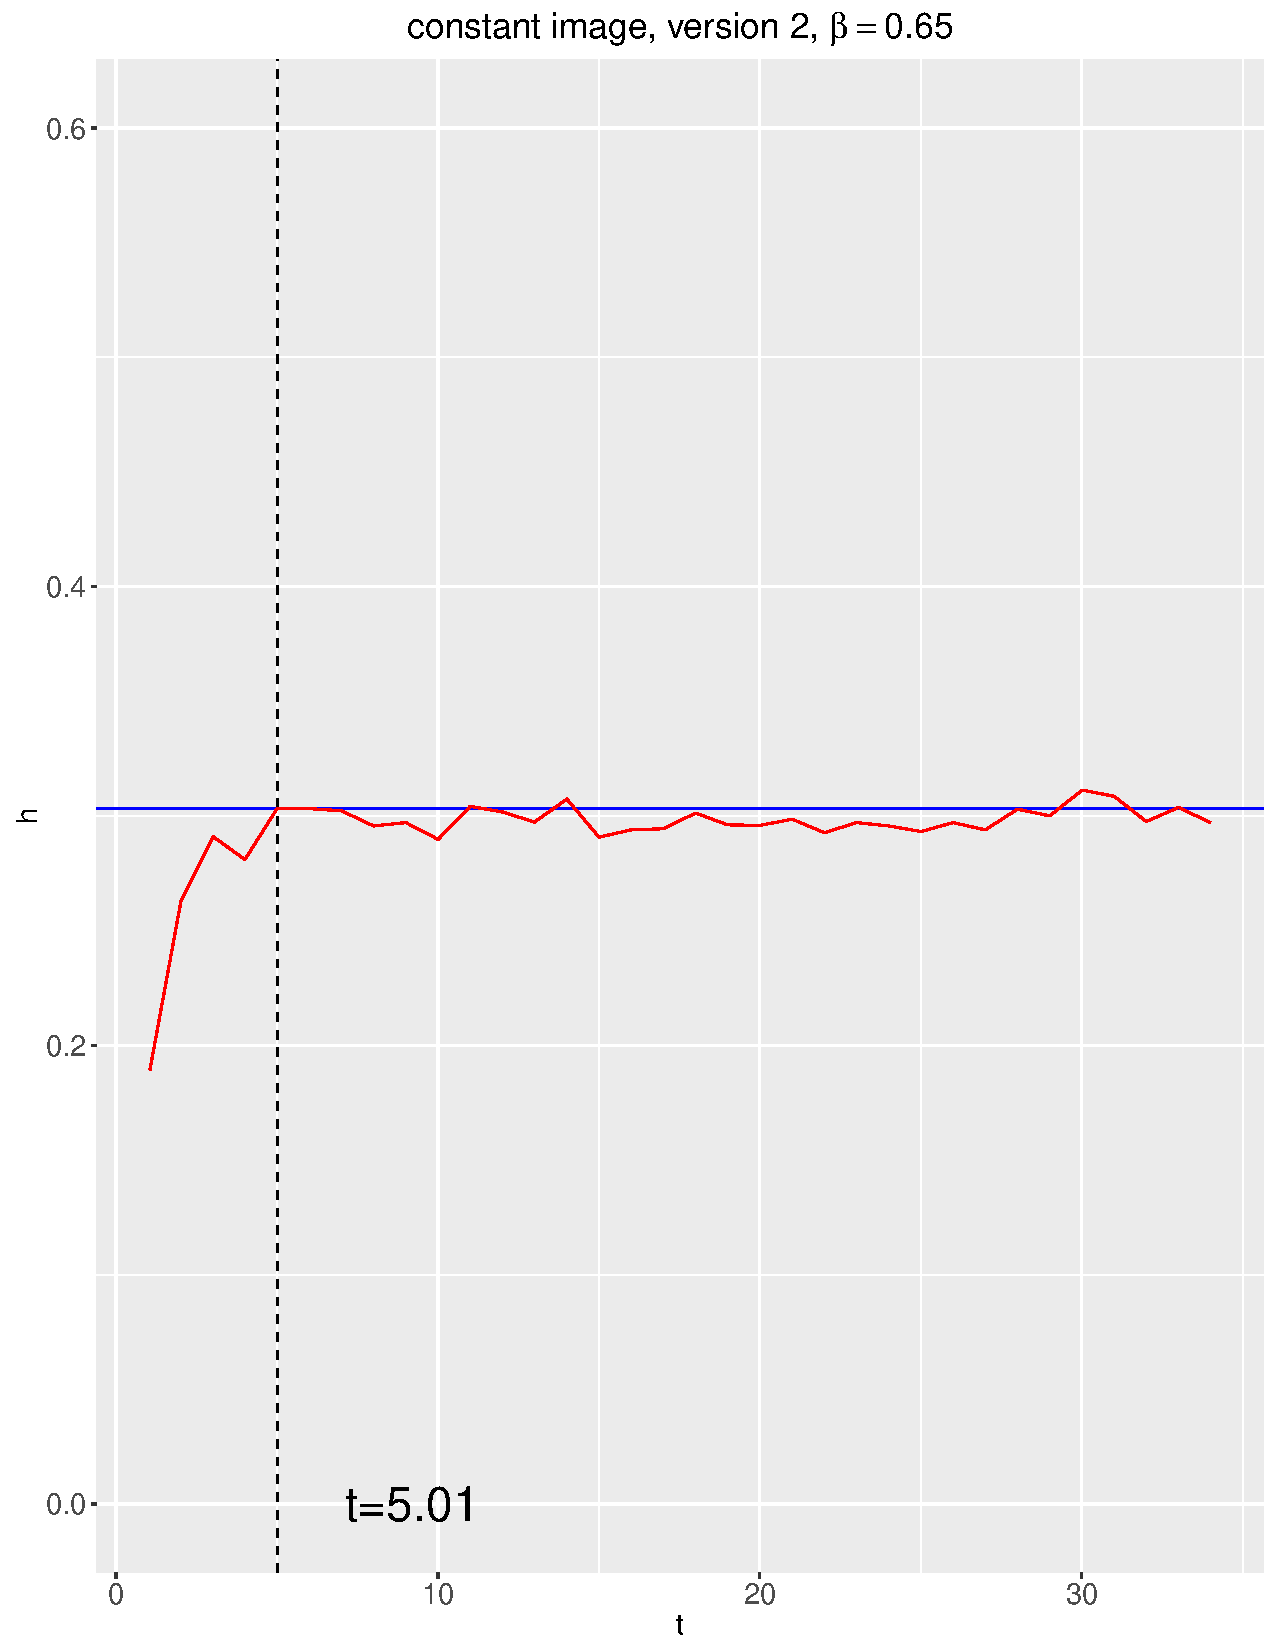
\includegraphics[width=\textwidth, height=0.32\textheight]{const_v2_65.pdf}
        \end{subfigure}
        \quad
        \begin{subfigure}[b]{0.475\textwidth}
            \centering
            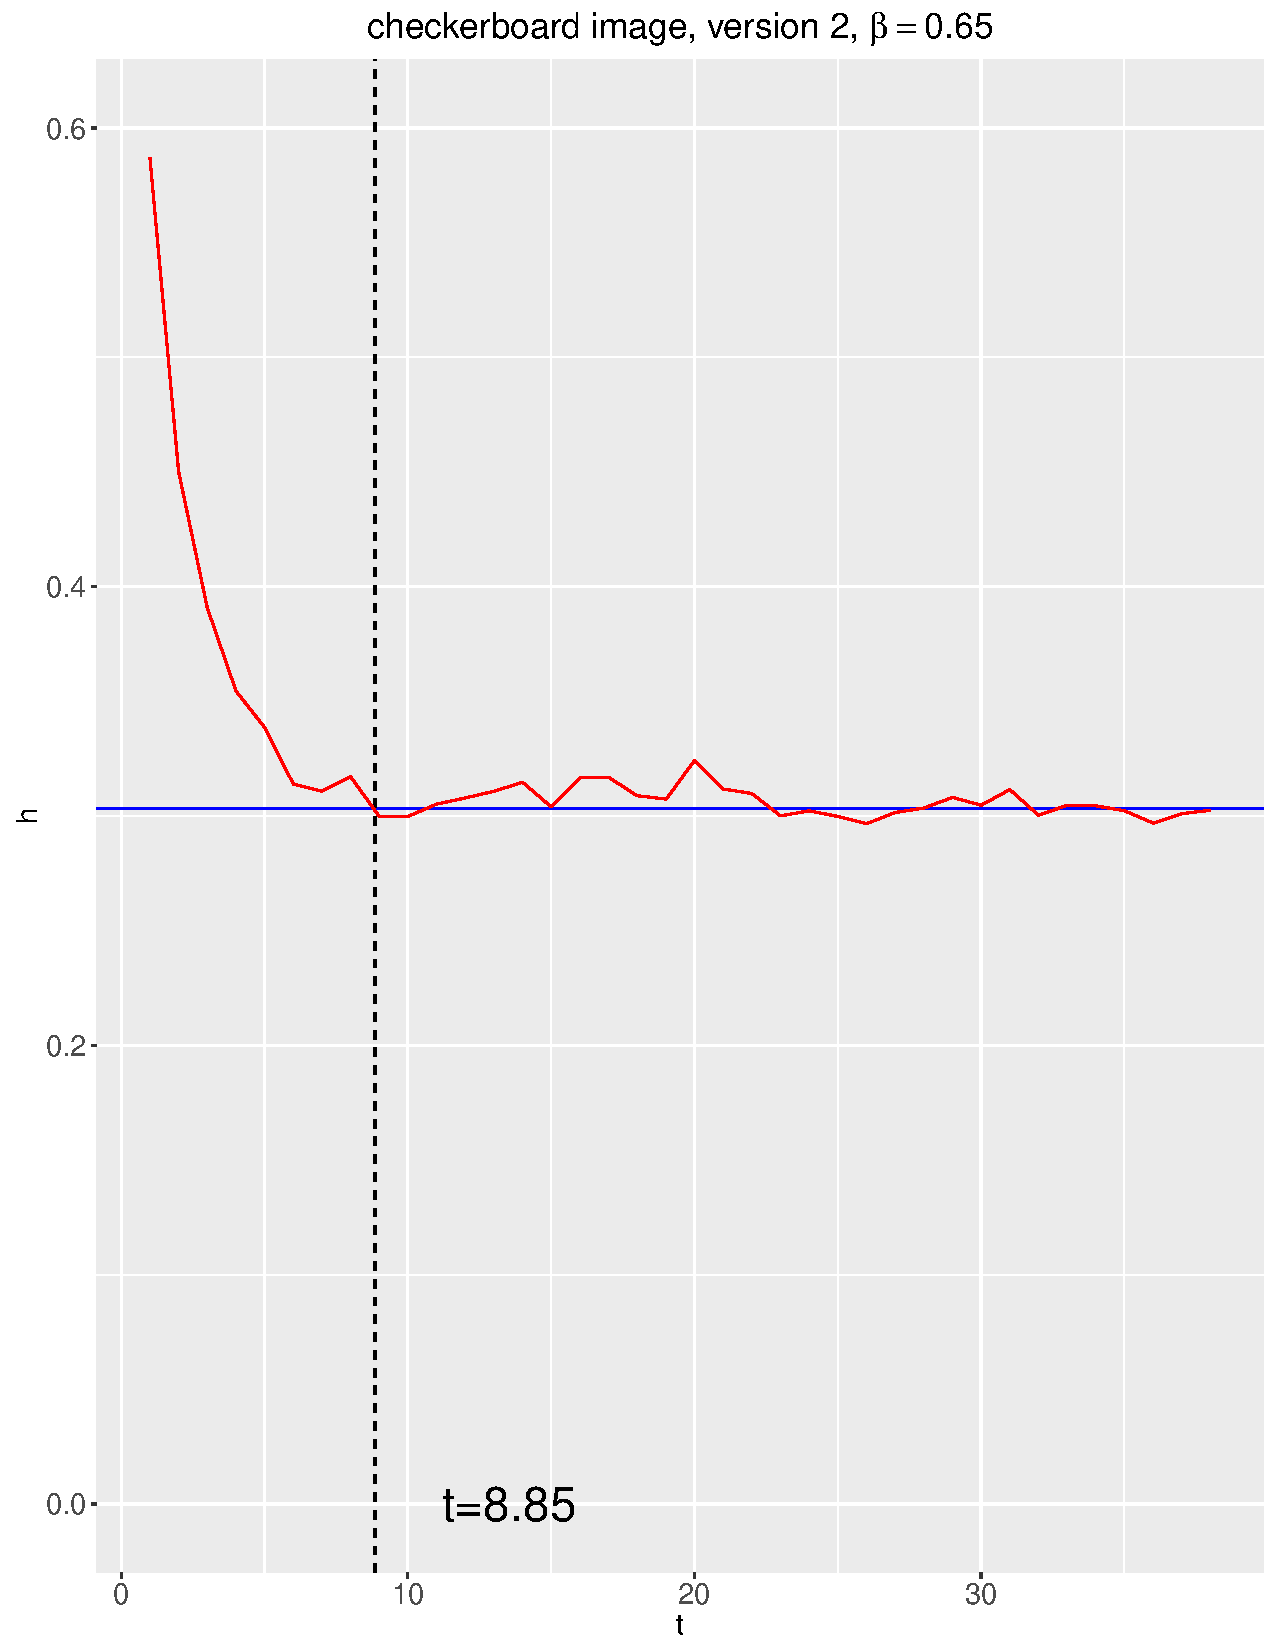
\includegraphics[width=\textwidth, height=0.32\textheight]{check_v2_65.pdf}
        \end{subfigure} \\
        \centering
        \begin{subfigure}[b]{0.475\textwidth}
            \centering
            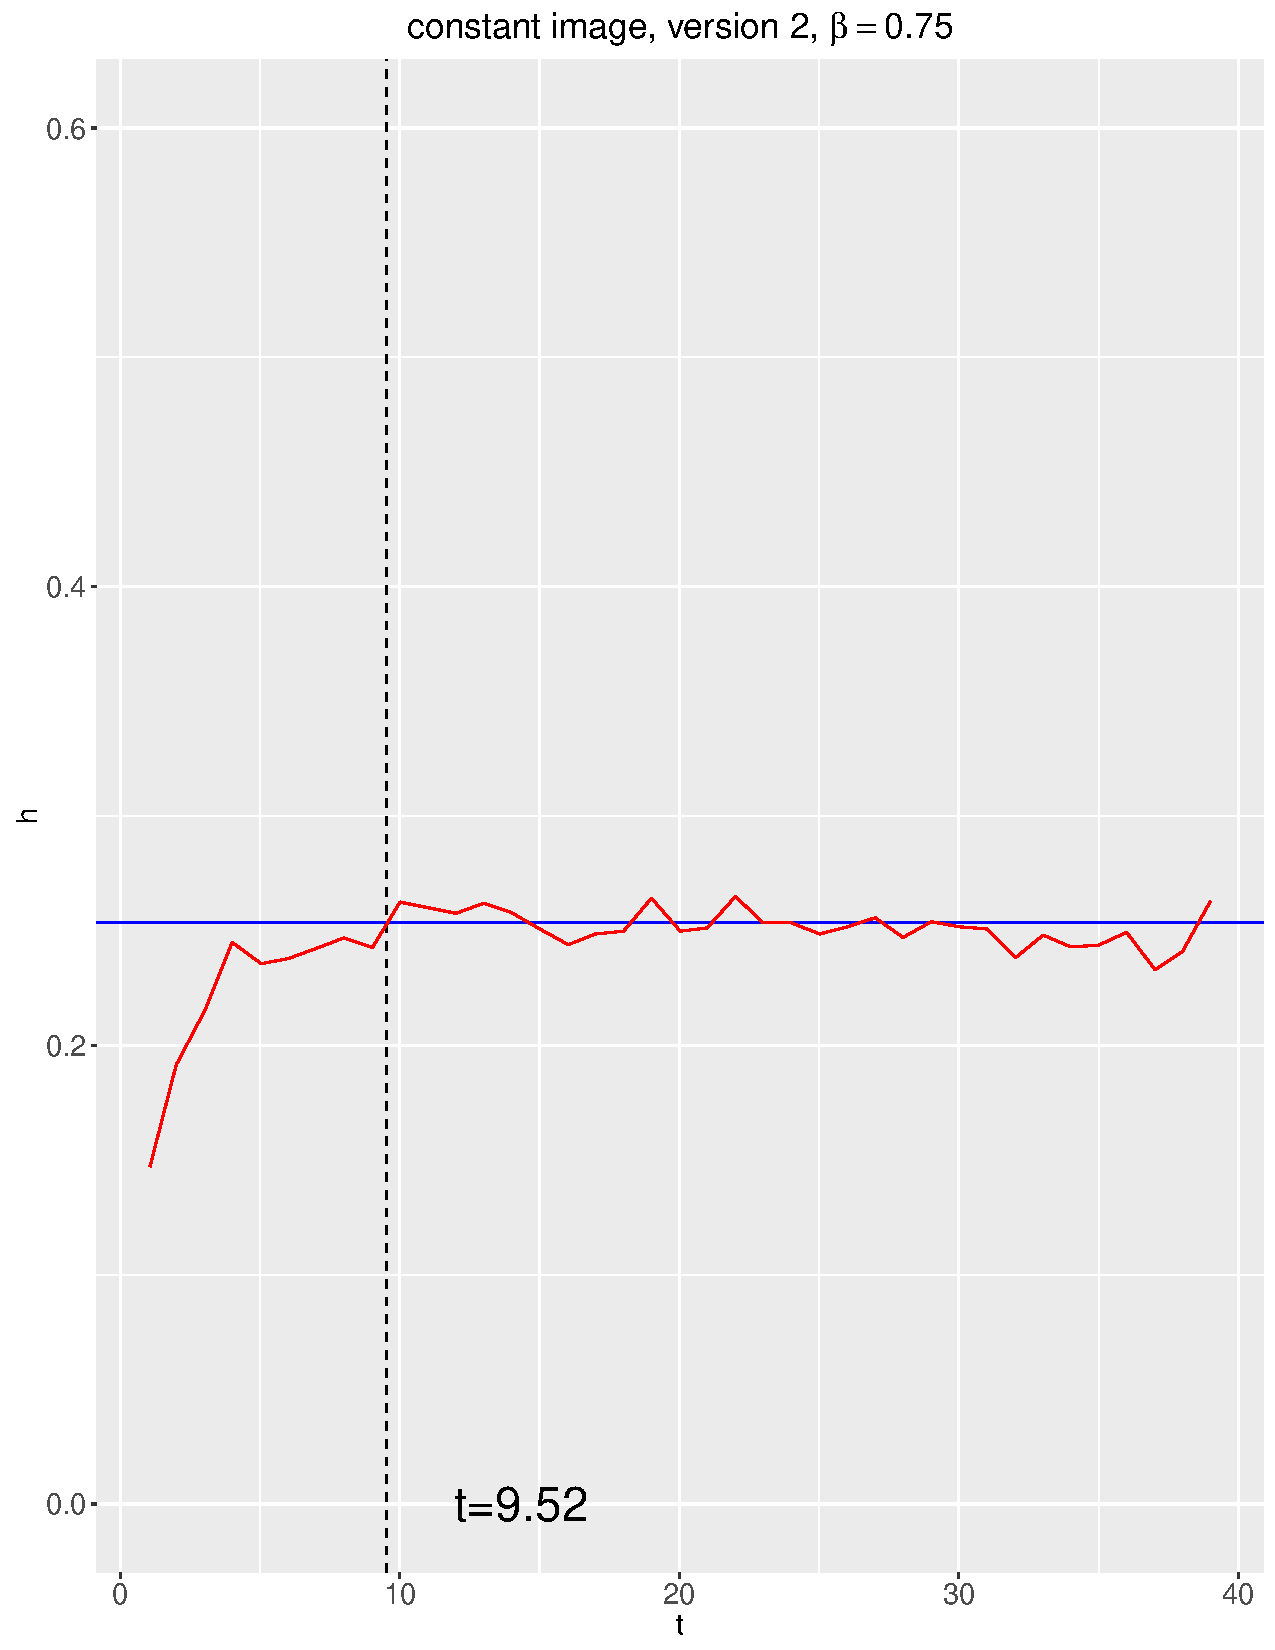
\includegraphics[width=\textwidth, height=0.32\textheight]{const_v2_75.pdf}
        \end{subfigure}
        \quad
        \begin{subfigure}[b]{0.475\textwidth}
            \centering
            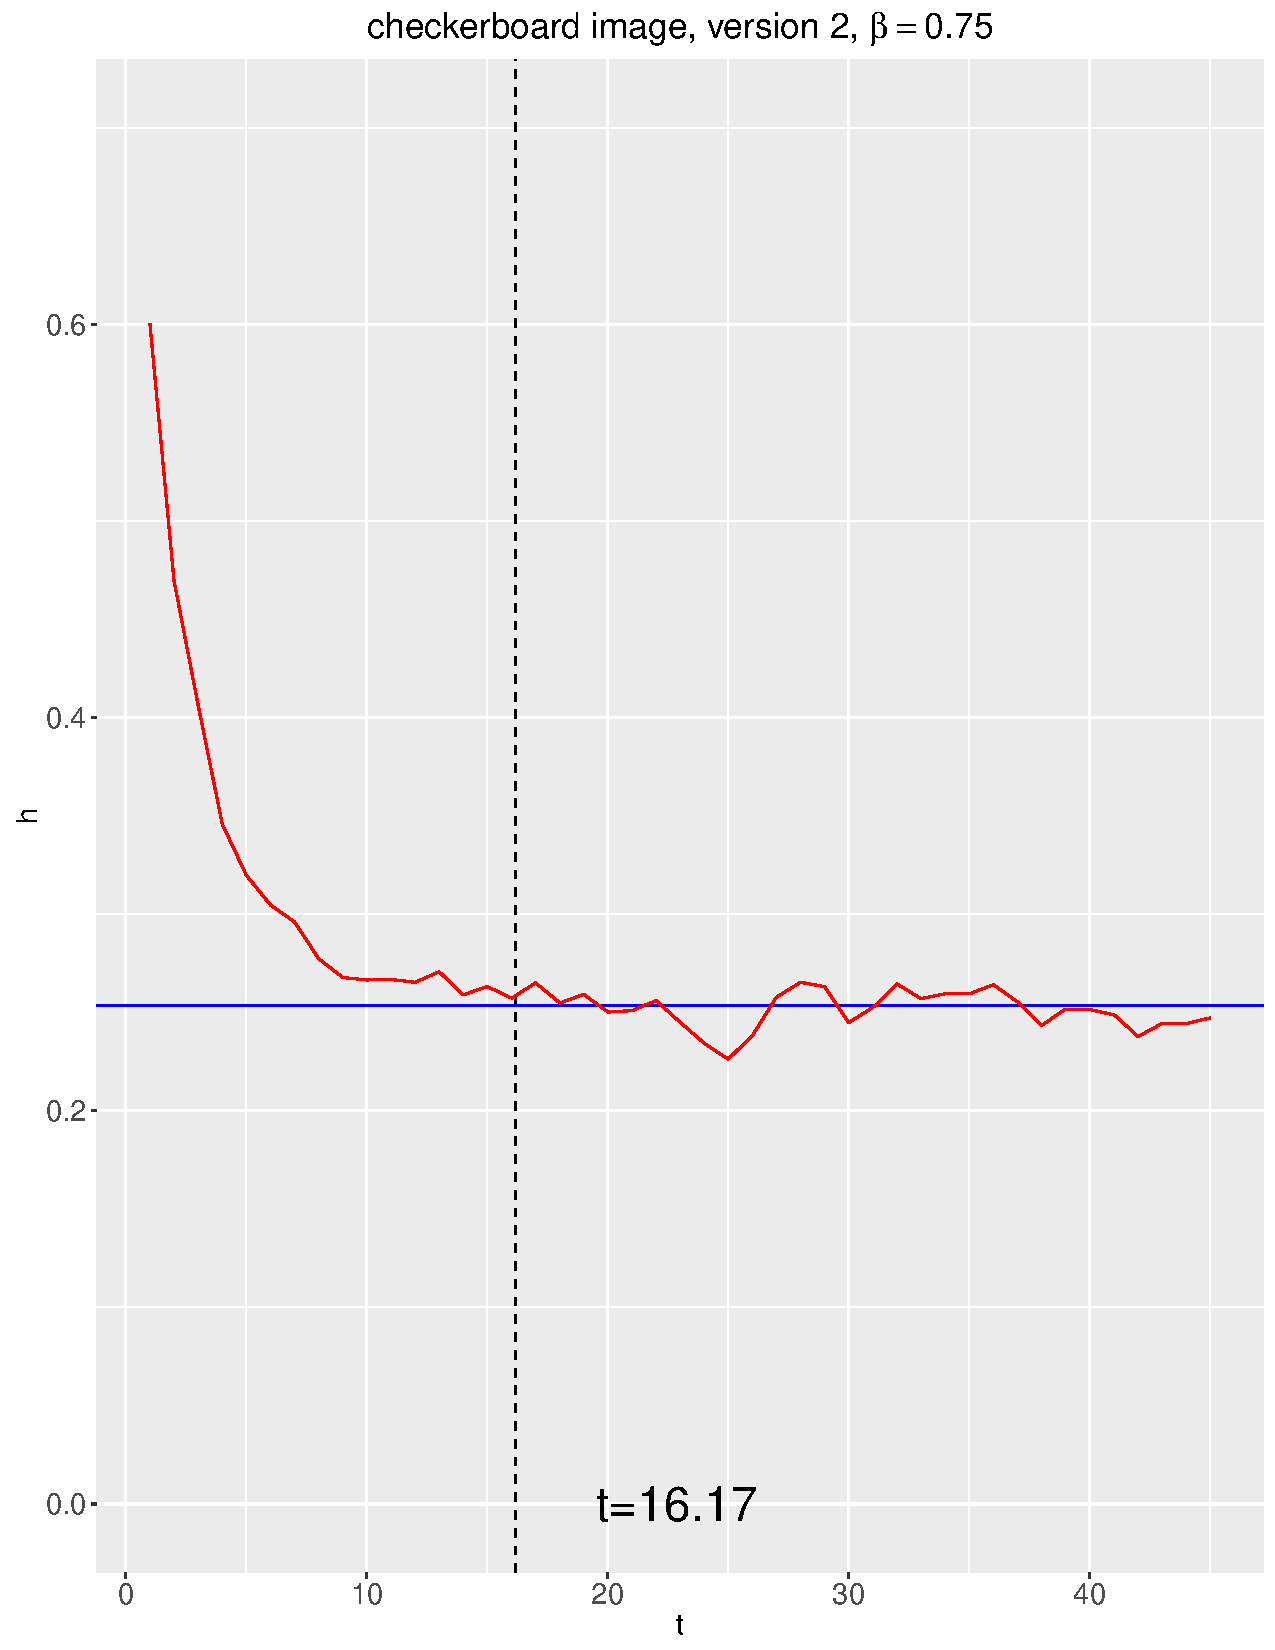
\includegraphics[width=\textwidth, height=0.32\textheight]{check_v2_75.pdf}
        \end{subfigure} \\
        \begin{subfigure}[b]{0.475\textwidth}
            \centering
            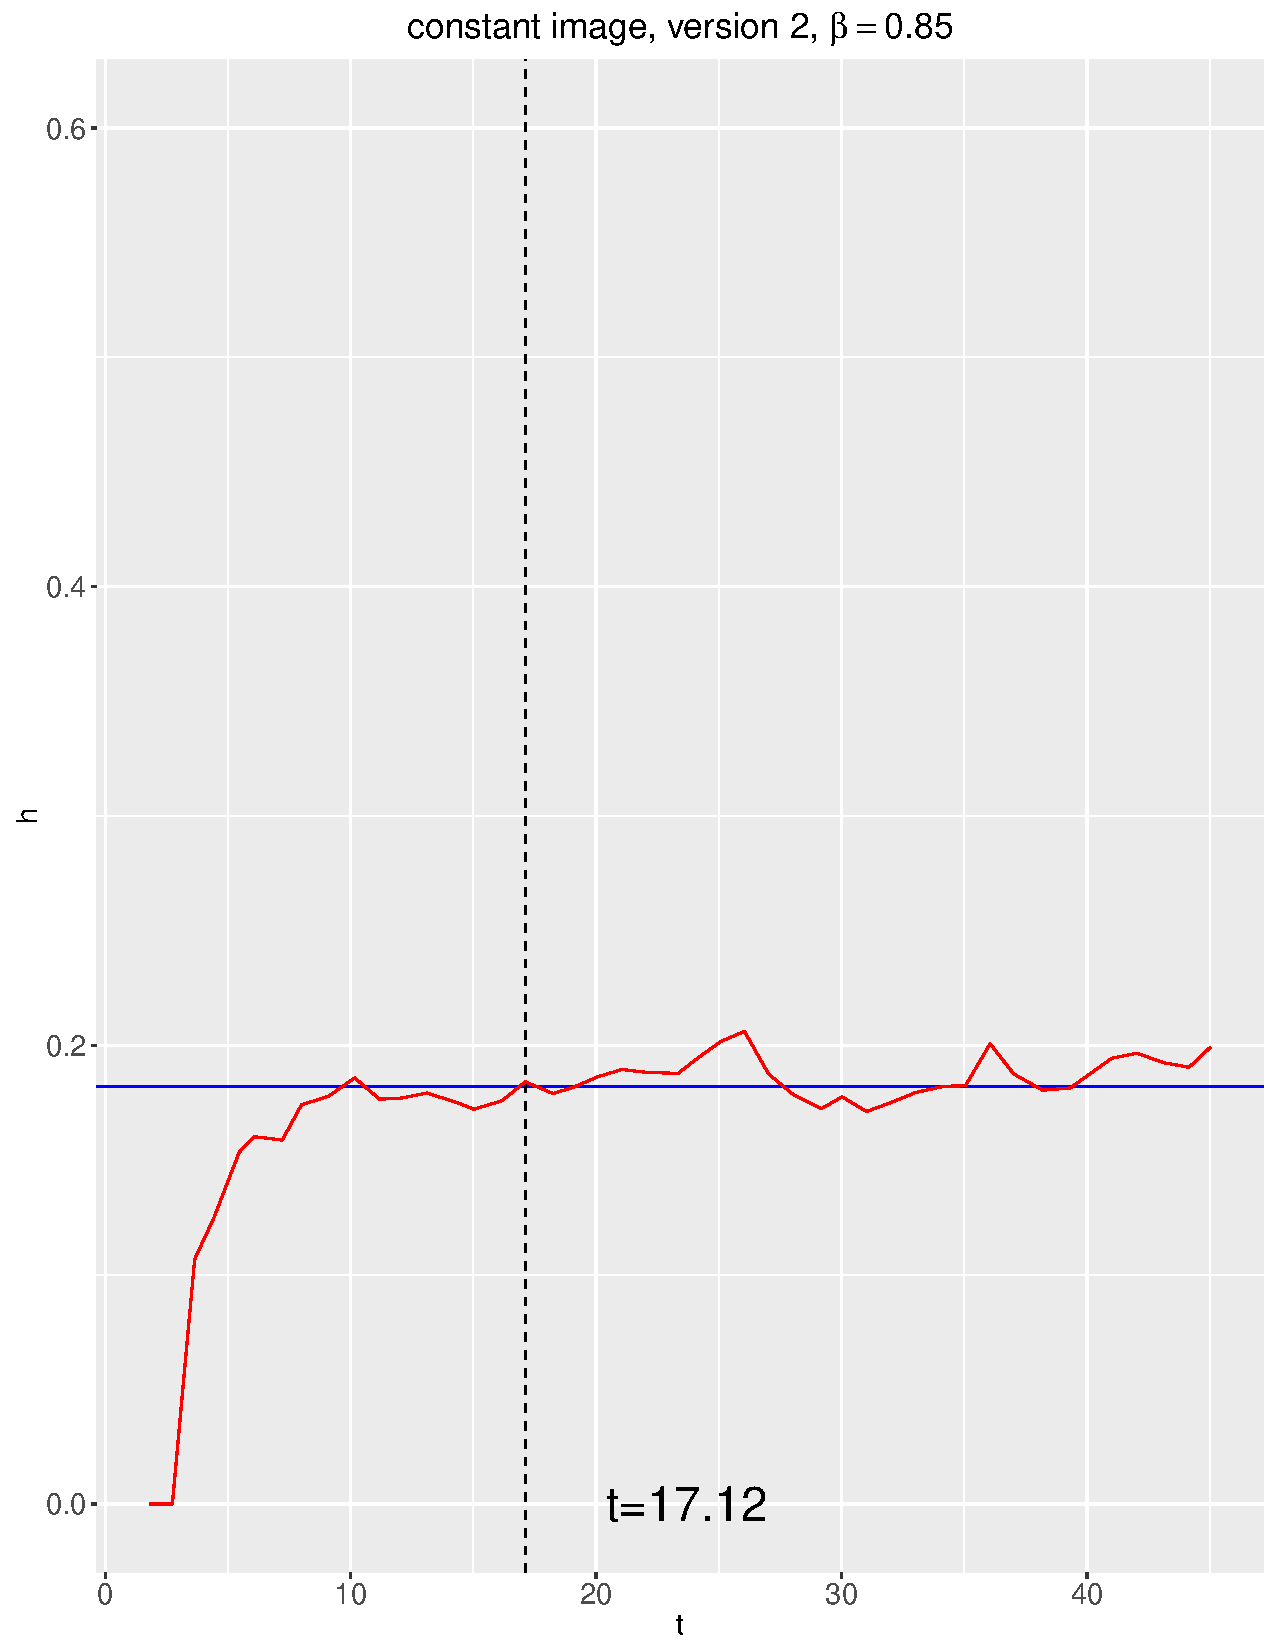
\includegraphics[width=\textwidth, height=0.32\textheight]{const_v2_85.pdf}
        \end{subfigure}
        \quad
        \begin{subfigure}[b]{0.475\textwidth}
            \centering
            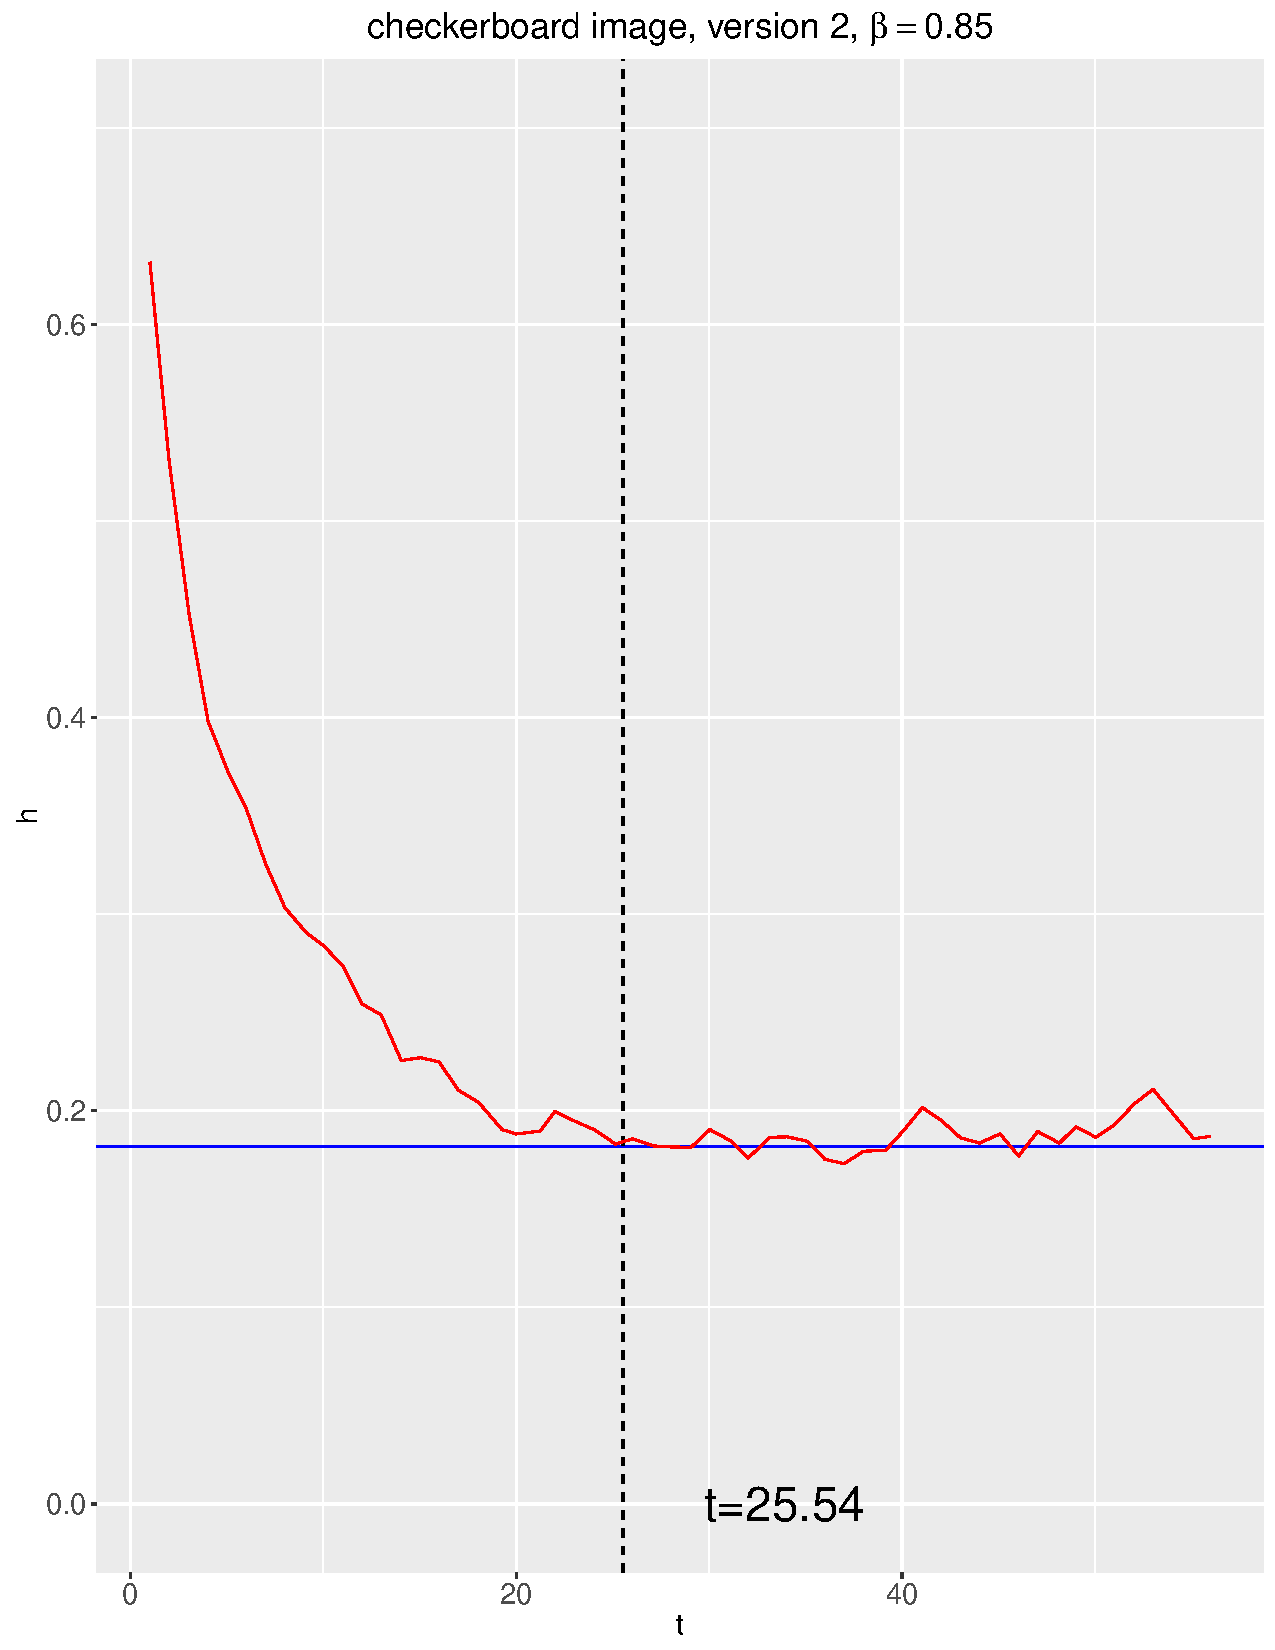
\includegraphics[width=\textwidth, height=0.32\textheight]{check_v2_85.pdf}
        \end{subfigure}
\end{figure}
\vspace{1cm}
P3\\
The bigger $\beta$ is, the lower average size of clusters is.
\begin{figure}[H]
            \centering
            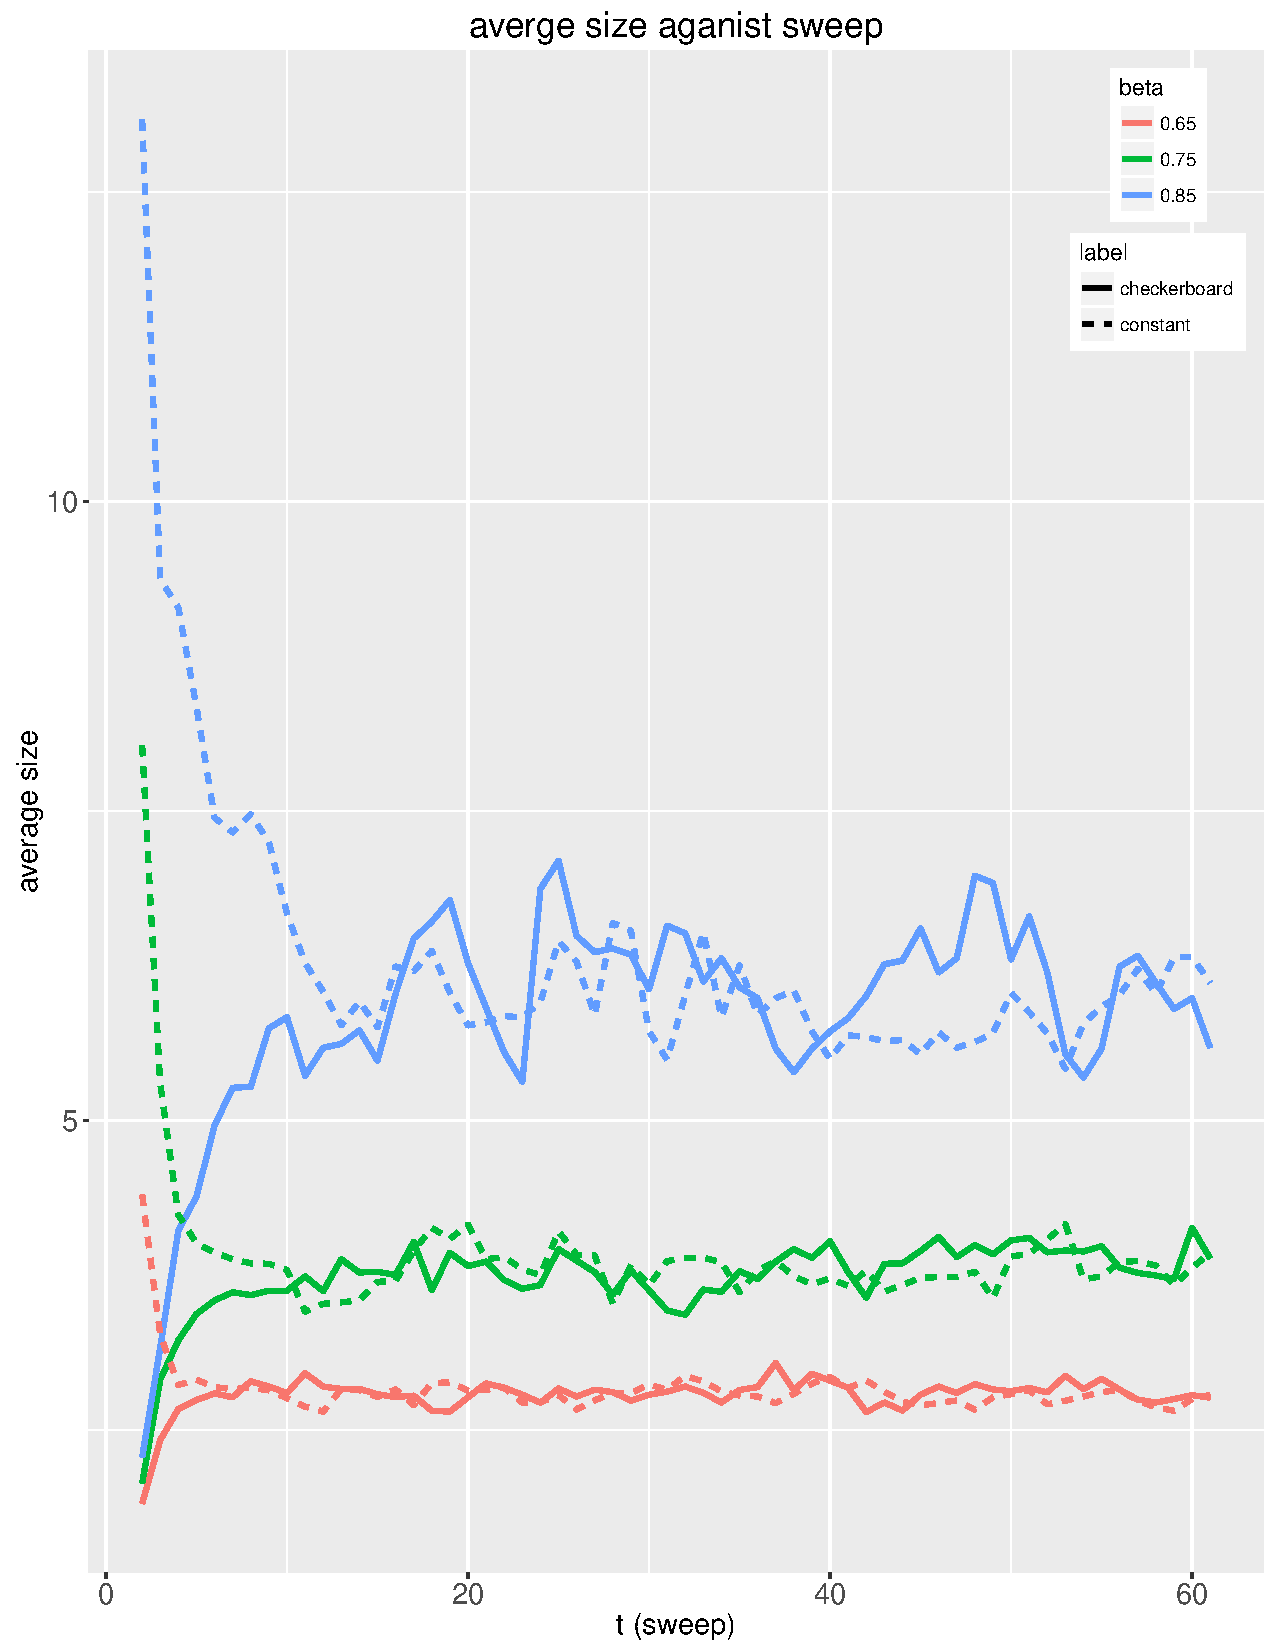
\includegraphics[width=0.8\textwidth, height=0.4\textheight]{size.pdf}
\end{figure}
P4\\
It converges very fast and only takes about 52 sweeps.
\begin{figure}[H]
        \centering
        \begin{subfigure}[b]{0.475\textwidth}
            \centering
            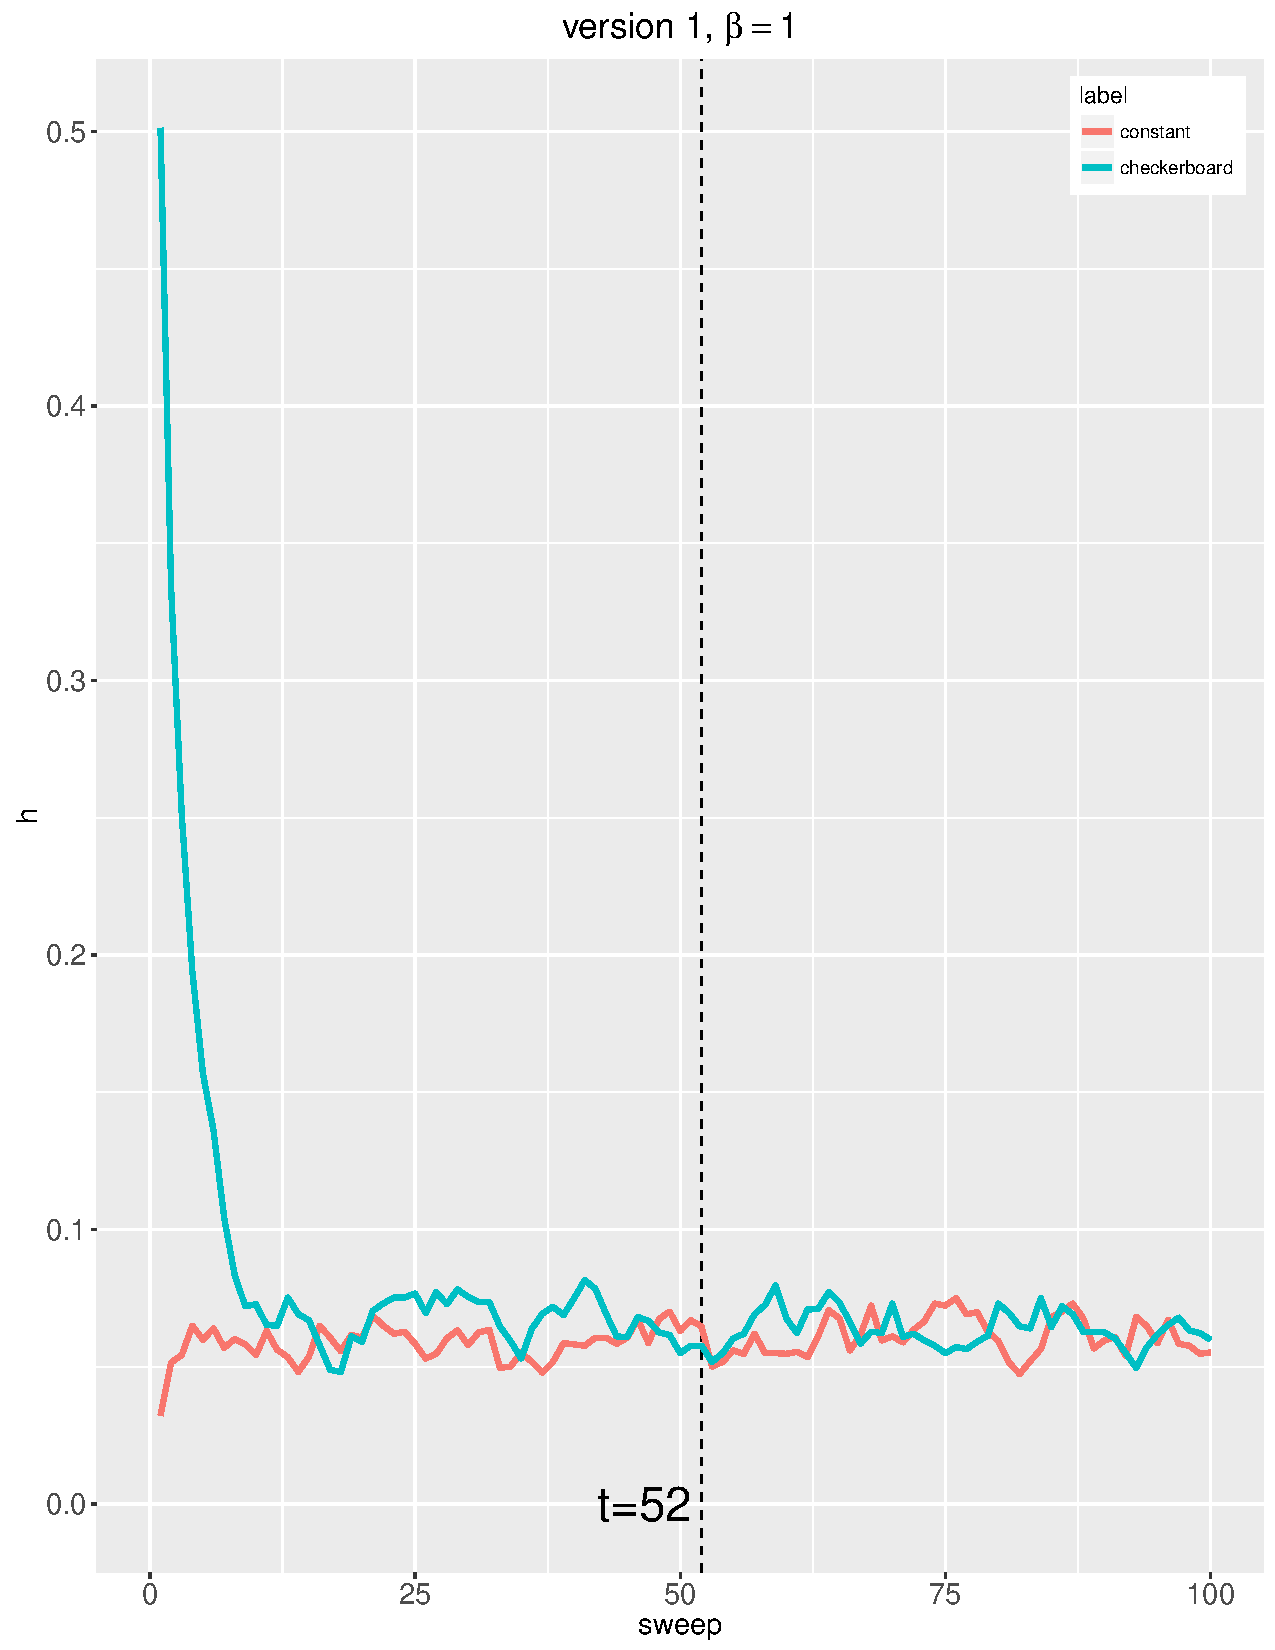
\includegraphics[width=\textwidth, height=0.32\textheight]{v1_1.pdf}
        \end{subfigure}
        \quad
        \begin{subfigure}[b]{0.475\textwidth}
            \centering
            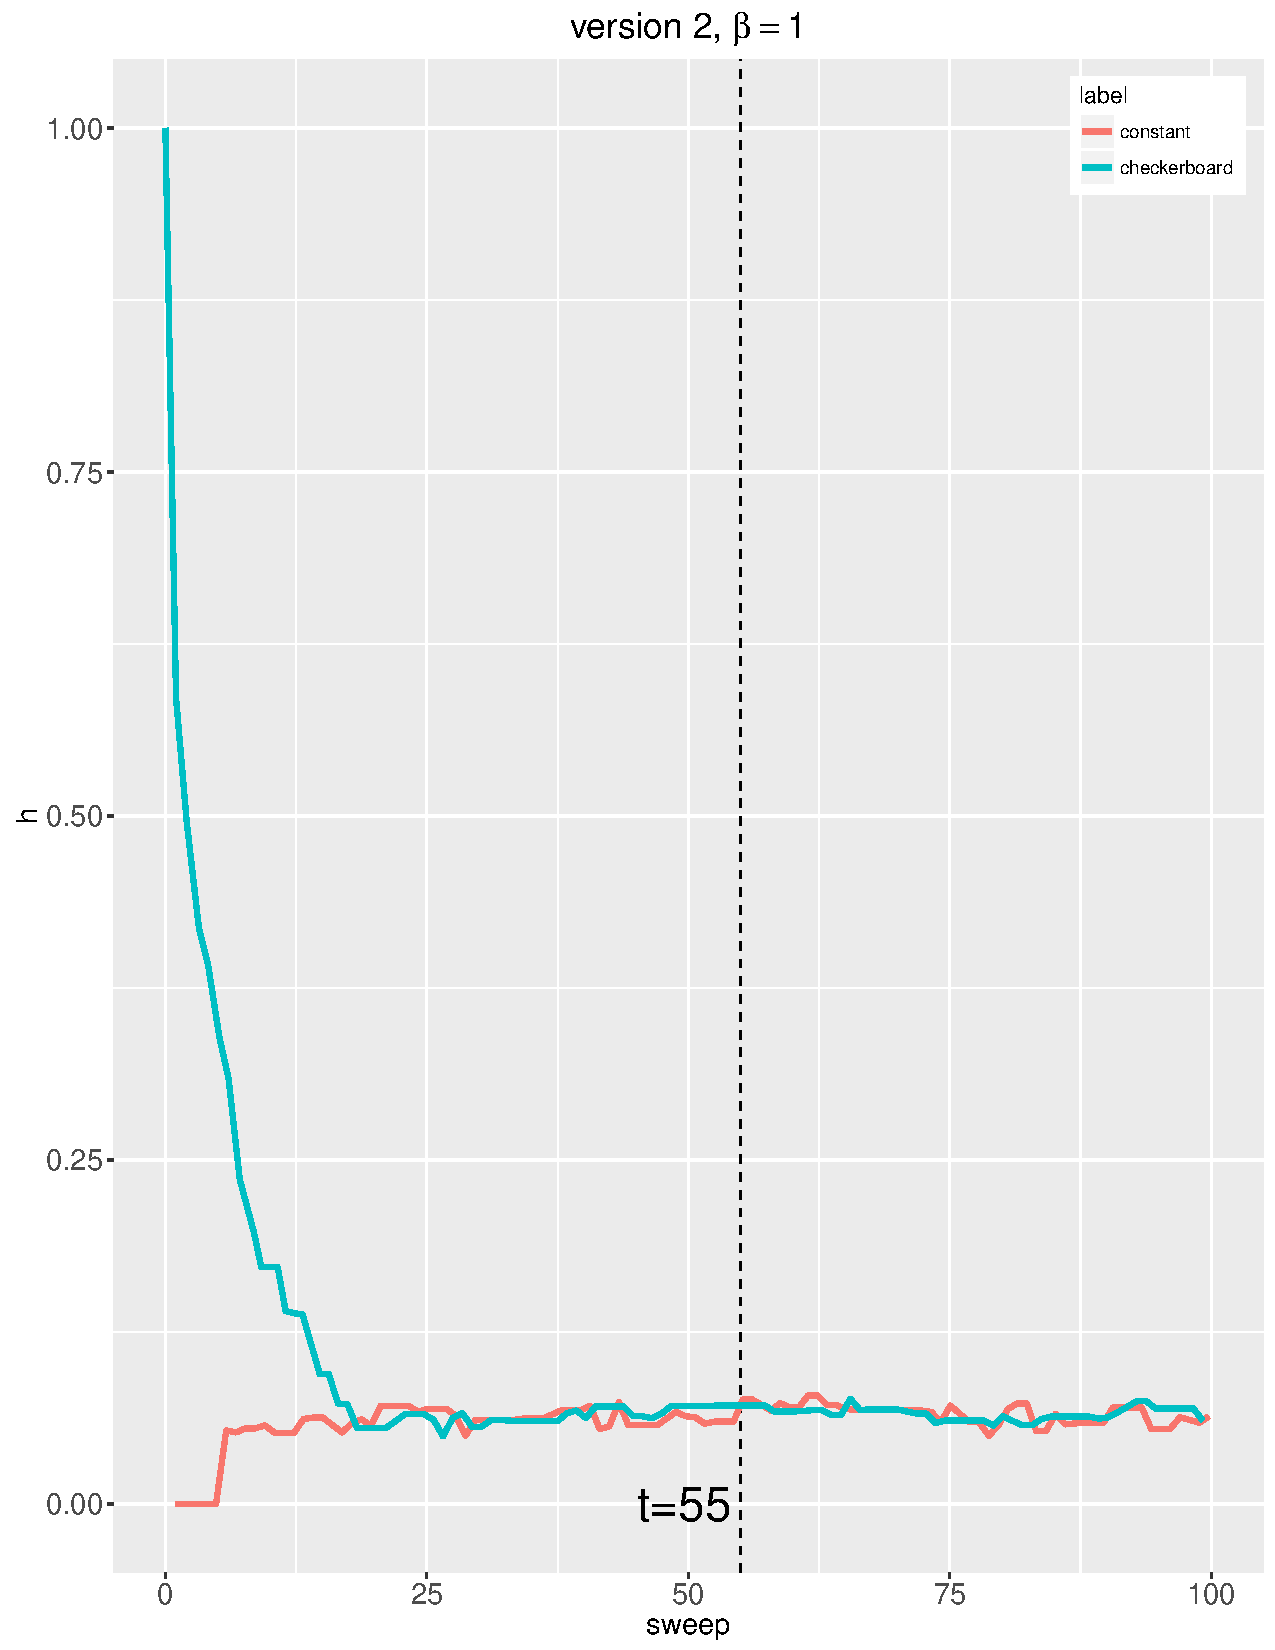
\includegraphics[width=\textwidth, height=0.32\textheight]{v2_1.pdf}
        \end{subfigure}
\end{figure}





\end{document}
